\newpage
\appendix

\section{Learning Curves}
\begin{figure}[hbt!]
\includegraphics[width=0.5\textwidth]{pics/accuracy_vs_epochs.png}
\caption{Model performance of ResNet20 on CIFAR100
during the training process for the reproductions.}%\label{tab:1a}
\end{figure}


\section{Reconstructions for cifar100, Default Attack Algorithm}\label{apx:rdaa}

\begin{figure}[hbt!]
\begin{subfigure}{.49\linewidth}\centering
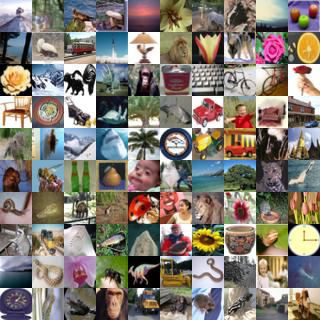
\includegraphics[width=\textwidth]{grids/data_cifar100_arch_ResNet20-4_epoch_200_optim_inversed_mode_normal_auglist__rlabel_False_ORIGINALS.png}
\caption{Inputs}%\label{tab:1a}
\end{subfigure}%
\hfill
\begin{subfigure}{.49\linewidth}\centering
\includegraphics[width=\textwidth]{grids/data_cifar100_arch_ResNet20-4_epoch_200_optim_inversed_mode_normal_auglist__rlabel_False_RECONSTRUCTIONS.png}
\caption{Reconstructions}%\label{tab:1a}
\end{subfigure}%
\caption{Inputs to the neural network (a) and reconstructions based on the gradients (b) for the unaugmented policy.}
    \label{fig:apprr}
\end{figure}


\begin{figure}[hbt!]
\begin{subfigure}{.49\linewidth}\centering
\includegraphics[width=\textwidth]{grids/data_cifar100_arch_ResNet20-4_epoch_200_optim_inversed_mode_aug_auglist_3-1-7_rlabel_False_ORIGINALS.png}
\caption{Inputs}%\label{tab:1a}
\end{subfigure}%
\hfill
\begin{subfigure}{.49\linewidth}\centering
\includegraphics[width=\textwidth]{grids/data_cifar100_arch_ResNet20-4_epoch_200_optim_inversed_mode_aug_auglist_3-1-7_rlabel_False_RECONSTRUCTIONS.png}
\caption{Reconstructions}%\label{tab:1a}
\end{subfigure}%
\caption{Inputs to the neural network (a) and reconstructions based on the gradients (b) for the \textit{3-1-7} policy.}
    \label{fig:apprr}
\end{figure}

\begin{figure}[hbt!]
\begin{subfigure}{.49\linewidth}\centering
\includegraphics[width=\textwidth]{grids/data_cifar100_arch_ResNet20-4_epoch_200_optim_inversed_mode_aug_auglist_43-18-18_rlabel_False_ORIGINALS.png}
\caption{Inputs}%\label{tab:1a}
\end{subfigure}%
\hfill
\begin{subfigure}{.49\linewidth}\centering
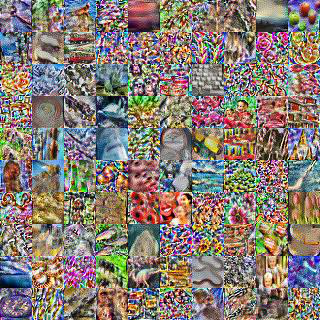
\includegraphics[width=\textwidth]{grids/data_cifar100_arch_ResNet20-4_epoch_200_optim_inversed_mode_aug_auglist_43-18-18_rlabel_False_RECONSTRUCTIONS.png}
\caption{Reconstructions}%\label{tab:1a}
\end{subfigure}%
\caption{Inputs to the neural network (a) and reconstructions based on the gradients (b) for the \textit{43-18-18} policy.}
    \label{fig:apprr}
\end{figure}



\begin{figure}[hbt!]
\begin{subfigure}{.49\linewidth}\centering
\includegraphics[width=\textwidth]{grids/data_cifar100_arch_ResNet20-4_epoch_200_optim_inversed_mode_aug_auglist_3-1-7+43-18-18_rlabel_False_ORIGINALS.png}
\caption{Inputs}%\label{tab:1a}
\end{subfigure}%
\hfill
\begin{subfigure}{.49\linewidth}\centering
\includegraphics[width=\textwidth]{grids/data_cifar100_arch_ResNet20-4_epoch_200_optim_inversed_mode_aug_auglist_3-1-7+43-18-18_rlabel_False_RECONSTRUCTIONS.png}
\caption{Reconstructions}%\label{tab:1a}
\end{subfigure}%
\caption{Inputs to the neural network (a) and reconstructions based on the gradients (b) for the \textit{Hybrid} policy.}
    \label{fig:apprr}
\end{figure}


\clearpage
\section{Reconstructions for cifar100, Enhanced Attack Algorithm}\label{apx:reaa}



\begin{figure}[hbt!]
\begin{subfigure}{.49\linewidth}\centering
\includegraphics[width=\textwidth]{grids/data_cifar100_arch_ResNet20-4_epoch_200_optim_inversed_mode_aug_auglist_3-1-7_rlabel_False_reaugment_translate_clipped1_ORIGINALS.png}
\caption{Inputs}%\label{tab:1a}
\end{subfigure}%
\hfill
\begin{subfigure}{.49\linewidth}\centering
\includegraphics[width=\textwidth]{grids/data_cifar100_arch_ResNet20-4_epoch_200_optim_inversed_mode_aug_auglist_3-1-7_rlabel_False_reaugment_translate_clipped1_RECONSTRUCTIONS.png}
\caption{Reconstructions}%\label{tab:1a}
\end{subfigure}%
\caption{Inputs to the neural network (a) and reconstructions based on the gradients (b) for the \textit{3-1-7} policy.}
    \label{fig:apprr}
\end{figure}


\begin{figure}[hbt!]
\begin{subfigure}{.49\linewidth}\centering
\includegraphics[width=\textwidth]{grids/data_cifar100_arch_ResNet20-4_epoch_200_optim_inversed_mode_aug_auglist_43-18-18_rlabel_False_reaugment_translate_clipped2_ORIGINALS.png}
\caption{Inputs}%\label{tab:1a}
\end{subfigure}%
\hfill
\begin{subfigure}{.49\linewidth}\centering
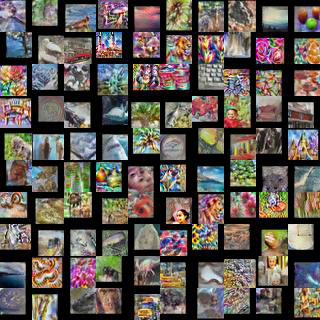
\includegraphics[width=\textwidth]{grids/data_cifar100_arch_ResNet20-4_epoch_200_optim_inversed_mode_aug_auglist_43-18-18_rlabel_False_reaugment_translate_clipped2_RECONSTRUCTIONS.png}
\caption{Reconstructions}%\label{tab:1a}
\end{subfigure}%
\caption{Inputs to the neural network (a) and reconstructions based on the gradients (b) for the \textit{43-18-18} policy.}
    \label{fig:apprr}
\end{figure}


\begin{figure}[hbt!]
\begin{subfigure}{.49\linewidth}\centering
\includegraphics[width=\textwidth]{grids/data_cifar100_arch_ResNet20-4_epoch_200_optim_inversed_mode_aug_auglist_3-1-7+43-18-18_rlabel_False_reaugment_translate_clipped3_ORIGINALS.png}
\caption{Inputs}%\label{tab:1a}
\end{subfigure}%
\hfill
\begin{subfigure}{.49\linewidth}\centering
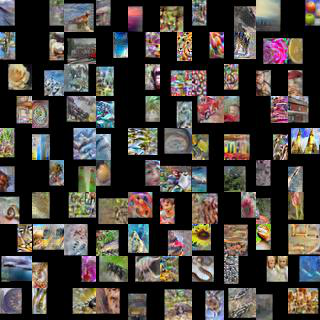
\includegraphics[width=\textwidth]{grids/data_cifar100_arch_ResNet20-4_epoch_200_optim_inversed_mode_aug_auglist_3-1-7+43-18-18_rlabel_False_reaugment_translate_clipped3_RECONSTRUCTIONS.png}
\caption{Reconstructions}%\label{tab:1a}
\end{subfigure}%
\caption{Inputs to the neural network (a) and reconstructions based on the gradients (b) for the \textit{Hybrid} policy.}
    \label{fig:apprr}
\end{figure}

